%!TEX root = CooperBarba2014.tex



We express the system of partial-differential equations in  \eqref{eq:pde} by the corresponding integral equations along the interface and the nanosurface, $\Gamma_1$ and $\Gamma_2$. Many authors have used the boundary-integral representation of the implicit-solvent model to compute solvation energies of proteins \cite{YoonLenhoff1990, Juffer1991a, LuETal2006, BajajETal2011, AltmanBardhanWhiteTidor09, GengKrasny2013, CooperBardhanBarba2013}, but apart from work led by Lenhoff \cite{YoonLenhoff1992}, we know of no studies that account for interacting surfaces in the system. 

Consider the setting in Figure \ref{fig:molecule_surface} with prescribed potential at $\Gamma_2$. The application of Green's second identity on the first two equations of \eqref{eq:pde} yields:
%
\begin{align} \label{eq:green_identity}
\phi_{1}+ K_{L}^{\Omega_1}(\phi_{1,\Gamma_1}) -  V_{L}^{\Omega_1} \left(\frac{\partial}{\partial \mathbf{n}}  \phi_{1,\Gamma_1}  \right) &  = \nonumber\\
 \frac{1}{\epsilon_1} \sum_{k=0}^{N_q}  \frac{q_k}{4\pi|\mathbf{r}_{\Omega_1} - \mathbf{r}_k|} &  \quad \text{on $\Omega_1$,} \nonumber \\ \nonumber \\
\phi_{2} - K_{Y}^{\Omega_2}(\phi_{2,\Gamma_1}) + V_{Y}^{\Omega_2} \left( \frac{\partial}{\partial \mathbf{n}} \phi_{2,\Gamma_1} \right) - & K_{Y}^{\Omega_2}(\phi_{2,\Gamma_2})  \nonumber \\
 + V_{Y}^{\Omega_2}  \left( \frac{\partial}{\partial \mathbf{n}} \phi_{2,\Gamma_2} \right) & = 0 \quad \text{on $\Omega_2$,}
\end{align}

\noindent where $\phi_{i,\Gamma_j} = \phi_i(\mathbf{r}_{\Gamma_j})$ is the potential in region $\Omega_i$ evaluated at the surface $\Gamma_j$. $K$ and $V$ are defined as

%
\begin{align} \label{eq:layers}
K_{L/Y}^{\Omega_i}(\phi_{i,\Gamma_j}) &= \oint_{\Gamma_j} \frac{\partial}{\partial \mathbf{n}} \left[ G_{L/Y}(\mathbf{r}_{\Omega_i},\mathbf{r}_{\Gamma_j}) \right]\phi_{i,\Gamma_j} \, \mathrm{d} \Gamma, \nonumber \\
V_{L/Y}^{\Omega_i} \left( \frac{\partial}{\partial \mathbf{n}} \phi_{i,\Gamma_j} \right) &= \oint_{\Gamma_j} \frac{\partial}{\partial \mathbf{n}} \phi_{i,\Gamma_j} G_{L/Y}(\mathbf{r}_{\Omega_i},\mathbf{r}_{\Gamma_j})  \, \mathrm{d} \Gamma,
\end{align}

\noindent corresponding to the double- and single-layer potentials of $\phi_{i,\Gamma_j}$ and $\frac{\partial}{\partial \mathbf{n}} \phi_{i,\Gamma_j}$ evaluated in the region $\Omega_i$. The functions $G_L$ and $G_Y$ are the free-space Green's functions of the Poisson (Laplace kernel) and linearized Poisson-Boltzmann (Yukawa kernel) equations, respectively:

\begin{align} \label{eq:free-space}
G_L(\mathbf{r}_{\Omega_1},\mathbf{r}_{\Gamma_1}) &= \frac{1}{4\pi|\mathbf{r}_{\Omega_1} - \mathbf{r}_{\Gamma_1}|}, \nonumber \\
G_Y(\mathbf{r}_{\Omega_2},\mathbf{r}_{\Gamma_2}) &= \frac{\exp \left( -\kappa |\mathbf{r}_{\Omega_1} - \mathbf{r}_{\Gamma_1}|\right)}{4\pi|\mathbf{r}_{\Omega_1} - \mathbf{r}_{\Gamma_1}|}.
\end{align}

\noindent We then take the limits 
$\mathbf{r}_{\Omega_1}\!\to\!\mathbf{r}_{\Gamma_1}$, 
$\mathbf{r}_{\Omega_2}\!\to\!\mathbf{r}_{\Gamma_1}$, 
$\mathbf{r}_{\Omega_2}\!\to\!\mathbf{r}_{\Gamma_2}$ on Equation \eqref{eq:green_identity}, and apply the boundary conditions:
$\phi_{1,\Gamma_1} = \phi_{2,\Gamma_1}$, 
$\epsilon_1\frac{\partial}{\partial \mathbf{n}} \phi_{1,\Gamma_1} =  \epsilon_2\frac{\partial}{\partial \mathbf{n}} \phi_{2,\Gamma_1} $ 
and $\phi_{2,\Gamma_2} = \phi_0$ to get the following system of boundary equations:

\vspace{1em}

%
%\begin{widetext}
\begin{align} \label{eq:integral_eq}
\frac{\phi_{1,\Gamma_1}}{2}+ K_{L}^{\Gamma_1}(\phi_{1,\Gamma_1}) - &V_{L}^{\Gamma_1} \left(\frac{\partial}{\partial \mathbf{n}}\phi_{1,\Gamma_1} \right)\nonumber\\  
&= \frac{1}{\epsilon_1} \sum_{k=0}^{N_q} \frac{q_k}{4\pi|\mathbf{r}_{\Gamma_1} - \mathbf{r}_k|}  \quad \text{on $\Gamma_1$,} \nonumber \\ 
\frac{\phi_{1,\Gamma_1}}{2} - K_{Y}^{\Gamma_1}(\phi_{1,\Gamma_1}) +  &\frac{\epsilon_1}{\epsilon_2} V_{Y}^{\Gamma_1} \left( \frac{\partial}{\partial \mathbf{n}} \phi_{1,\Gamma_1} \right)\nonumber \\ 
- K_{Y}^{\Gamma_1}&(\phi_{0})  + V_{Y}^{\Gamma_1} \left( \frac{\partial}{\partial \mathbf{n}} \phi_{2,\Gamma_2} \right)  = 0 \quad \text{on $\Gamma_1$,} \nonumber \\ 
- K_{Y}^{\Gamma_2}(\phi_{1,\Gamma_1}) + \frac{\epsilon_1}{\epsilon_2} V_{Y}^{\Gamma_2} &\left( \frac{\partial}{\partial \mathbf{n}} \phi_{1,\Gamma_1} \right)\nonumber \\ 
+ \frac{\phi_{0}}{2} - &K_{Y}^{\Gamma_2}(\phi_{0}) +  V_{Y}^{\Gamma_2} \left( \frac{\partial}{\partial \mathbf{n}} \phi_{2,\Gamma_2} \right)  = 0 \quad \text{on $\Gamma_2$.}
\end{align}
%\end{widetext}


\noindent Rearranging terms, we write Equation \eqref{eq:integral_eq} in matrix form, as follows:
%
 \begin{align} \label{eq:matrix_phi}
 \left[
    \begin{matrix} % or pmatrix or bmatrix or Bmatrix or ...
       \frac{1}{2} + K_{L}^{\Gamma_1} & -V_{L}^{\Gamma_1} & 0 \vspace{0.2cm}\\
       \frac{1}{2} - K_{Y}^{\Gamma_1} &  \frac{\epsilon_1}{\epsilon_2} V_{Y}^{\Gamma_1} & V_{Y}^{\Gamma_1} \vspace{0.2cm} \\
       - K_{Y}^{\Gamma_2} & \frac{\epsilon_1}{\epsilon_2} V_{Y}^{\Gamma_2} & V_{Y}^{\Gamma_2} \\
    \end{matrix}
    \right] \left[ 
    \begin{matrix} % or pmatrix or bmatrix or Bmatrix or ...
       \phi_{1,\Gamma_1} \vspace{0.2cm} \\
       \frac{\partial}{\partial \mathbf{n}} \phi_{1,\Gamma_1} \vspace{0.2cm}\\
       \frac{\partial}{\partial \mathbf{n}} \phi_{2,\Gamma_2}\\
    \end{matrix} 
     \right] =  & \nonumber \\
    \left[
    \begin{matrix} % or pmatrix or bmatrix or Bmatrix or ...
       \sum_{k=0}^{N_q} \frac{q_k}{4\pi|\mathbf{r}_{\Gamma_1} - \mathbf{r}_k|} \vspace{0.2cm} \\
        K_{Y}^{\Gamma_1}(\phi_{0}) \vspace{0.2cm} \\
        -\left(\frac{1}{2} - K_{Y}^{\Gamma_2}\right) (\phi_0)
    \end{matrix}
    \right].
 \end{align}

\medskip
\noindent If the surface $\Gamma_2$ has prescribed charge, corresponding to a Neumann boundary condition, $-\epsilon_2\frac{\partial}{\partial \mathbf{n}} \phi_{2,\Gamma_2} = \sigma_0$, the equivalent derivation yields

 \begin{align} \label{eq:matrix_dphi}
 \left[
    \begin{matrix} % or pmatrix or bmatrix or Bmatrix or ...
       \frac{1}{2} + K_{L}^{\Gamma_1} & -V_{L}^{\Gamma_1} & 0 \vspace{0.2cm}\\
       \frac{1}{2} - K_{Y}^{\Gamma_1} &  \frac{\epsilon_1}{\epsilon_2} V_{Y}^{\Gamma_1} & -K_{Y}^{\Gamma_1} \vspace{0.2cm} \\
       - K_{Y}^{\Gamma_2} & \frac{\epsilon_1}{\epsilon_2} V_{Y}^{\Gamma_2} & \left(\frac{1}{2} - K_{Y}^{\Gamma_2}\right) \\
    \end{matrix}
    \right] \left[ 
    \begin{matrix} % or pmatrix or bmatrix or Bmatrix or ...
       \phi_{1,\Gamma_1} \vspace{0.2cm} \\
       \frac{\partial}{\partial \mathbf{n}} \phi_{1,\Gamma_1} \vspace{0.2cm}\\
       \phi_{2,\Gamma_2}\\
    \end{matrix} 
     \right] =   \nonumber \\
    \left[
    \begin{matrix} % or pmatrix or bmatrix or Bmatrix or ...
       \sum_{k=0}^{N_q} \frac{q_k}{4\pi|\mathbf{r}_{\Gamma_1} - \mathbf{r}_k|} \vspace{0.2cm} \\
        -V_{Y}^{\Gamma_1} \left( \frac{\partial}{\partial \mathbf{n}} \phi_{2,\Gamma_2} \right) \vspace{0.2cm} \\
        -V_{Y}^{\Gamma_2} \left( -\frac{\sigma_0}{\epsilon_2} \right)
    \end{matrix}
    \right].
 \end{align}
 
% \medskip

The formulation detailed in this section differs from the work by Lenhoff and co-workers \cite{YoonLenhoff1992,RothLenhoff1993} because they consider an infinite charged surface, modeled using a modified Green's function to account for the half-space domain. Lenhoff's approach has the advantage that the charged surface does not require a mesh, but cannot be applied to any situation where the surface has non-planar geometry. An infinite surface may not be a good model if the size of a device is comparable to the protein's, like it happens with nano-structures.
In that case, one needs to be able to represent the detailed geometry of a device via a surface mesh, and satisfy boundary conditions there, as detailed above.

The system in \eqref{eq:matrix_dphi} can be extended to account for Stern layers and solvent-filled cavities by adding more surfaces or interfaces. In our code, we deal with multiple surfaces in the manner presented by Altman and co-workers \cite{AltmanBardhanWhiteTidor09}, as described in our previous paper \cite{CooperBardhanBarba2013}.



%%%%===================================
%%%% Commented out section on multiple surfaces
 \begin{comment}
 
Figure \ref{fig:molecule_surface_stern} shows a more interesting situation. There, the surface $\Gamma_3$ has a given potential $\phi_0$ with a Stern layer, and interacts with a molecule that has a pocket of solvent, where the linearized Poisson-Boltzmann equation is enforced. In this case, the derivation that led to Equation \eqref{eq:matrix_phi} yields
 
 \newpage
 
 
% \begin{widetext}
  \begin{equation} \label{eq:matrix_stern}
 \left[
 %coefficient matrix
    \begin{matrix} % or pmatrix or bmatrix or Bmatrix or ...
       \frac{1}{2} + K_{Y}^{\Gamma_1} & -V_{Y}^{\Gamma_1} & 0  & 0 & 0 & 0 & 0\vspace{0.2cm}\\
       \frac{1}{2} - K_{L}^{\Gamma_1} &  \frac{\epsilon_1}{\epsilon_2} V_{L}^{\Gamma_1} & K_{L}^{\Gamma_1} & -V_{L}^{\Gamma_1} & 0 & 0 & 0 \vspace{0.2cm} \\
        -K_{L}^{\Gamma_2} &  \frac{\epsilon_1}{\epsilon_2} V_{L}^{\Gamma_2} & \frac{1}{2}+K_{L}^{\Gamma_2} & -V_{L}^{\Gamma_2} & 0 & 0 & 0 \vspace{0.2cm} \\
        0 & 0 & \frac{1}{2} - K_{Y}^{\Gamma_2} &  \frac{\epsilon_2}{\epsilon_4} V_{Y}^{\Gamma_2} & 0 & -K_{Y}^{\Gamma_2} &  \frac{\epsilon_3}{\epsilon_4} V_{Y}^{\Gamma_2} \vspace{0.2cm} \\
        0 & 0 & 0 & 0 & V_{L}^{\Gamma_3} & K_{L}^{\Gamma_3} & -V_{L}^{\Gamma_3} \vspace{0.2cm} \\
        0 & 0 & 0 & 0 & V_{L}^{\Gamma_4} & \frac{1}{2}+K_{L}^{\Gamma_4} & -V_{L}^{\Gamma_4} \vspace{0.2cm} \\
        0 & 0 & -K_{Y}^{\Gamma_4} &  \frac{\epsilon_2}{\epsilon_4} V_{Y}^{\Gamma_4} & 0 & \frac{1}{2} -K_{Y}^{\Gamma_4} &  \frac{\epsilon_3}{\epsilon_4} V_{Y}^{\Gamma_4} \vspace{0.2cm} \\
    \end{matrix}
    \right] %& \nonumber \\ 
    %vector of unknowns
   \cdot \left[ 
    \begin{matrix} % or pmatrix or bmatrix or Bmatrix or ...
       \phi_{1,\Gamma_1} \vspace{0.2cm} \\
       \frac{\partial}{\partial \mathbf{n}} \phi_{1,\Gamma_1} \vspace{0.2cm}\\
       \phi_{2,\Gamma_2} \vspace{0.2cm}\\
       \frac{\partial}{\partial \mathbf{n}} \phi_{2,\Gamma_2} \vspace{0.2cm}\\
       \frac{\partial}{\partial \mathbf{n}} \phi_{3,\Gamma_3} \vspace{0.2cm}\\
       \phi_{3,\Gamma_4} \vspace{0.2cm}\\
       \frac{\partial}{\partial \mathbf{n}} \phi_{3,\Gamma_4} \vspace{0.2cm}\\
    \end{matrix} 
     \right] 
     = 
     %right-hand-side  
    \left[
    \begin{matrix} % or pmatrix or bmatrix or Bmatrix or ...
        0 \vspace{0.2cm} \\
       \sum_{k=0}^{N_q} \frac{q_k}{4\pi|\mathbf{r}_{\Gamma_1} - \mathbf{r}_k|} \vspace{0.2cm} \\
       \sum_{k=0}^{N_q} \frac{q_k}{4\pi|\mathbf{r}_{\Gamma_2} - \mathbf{r}_k|} \vspace{0.2cm} \\
        0 \vspace{0.2cm} \\
        -\left(\frac{1}{2} - K_{L}^{\Gamma_3}\right) (\phi_{0}) \vspace{0.2cm} \\
        K_{L}^{\Gamma_3} \left( \phi_{0} \right) \vspace{0.2cm} \\
       0
    \end{matrix}
    \right] 
 \end{equation}
% \end{widetext}
 
 
 \begin{figure}[h] %  figure placement: here, top, bottom, or page
   \centering
   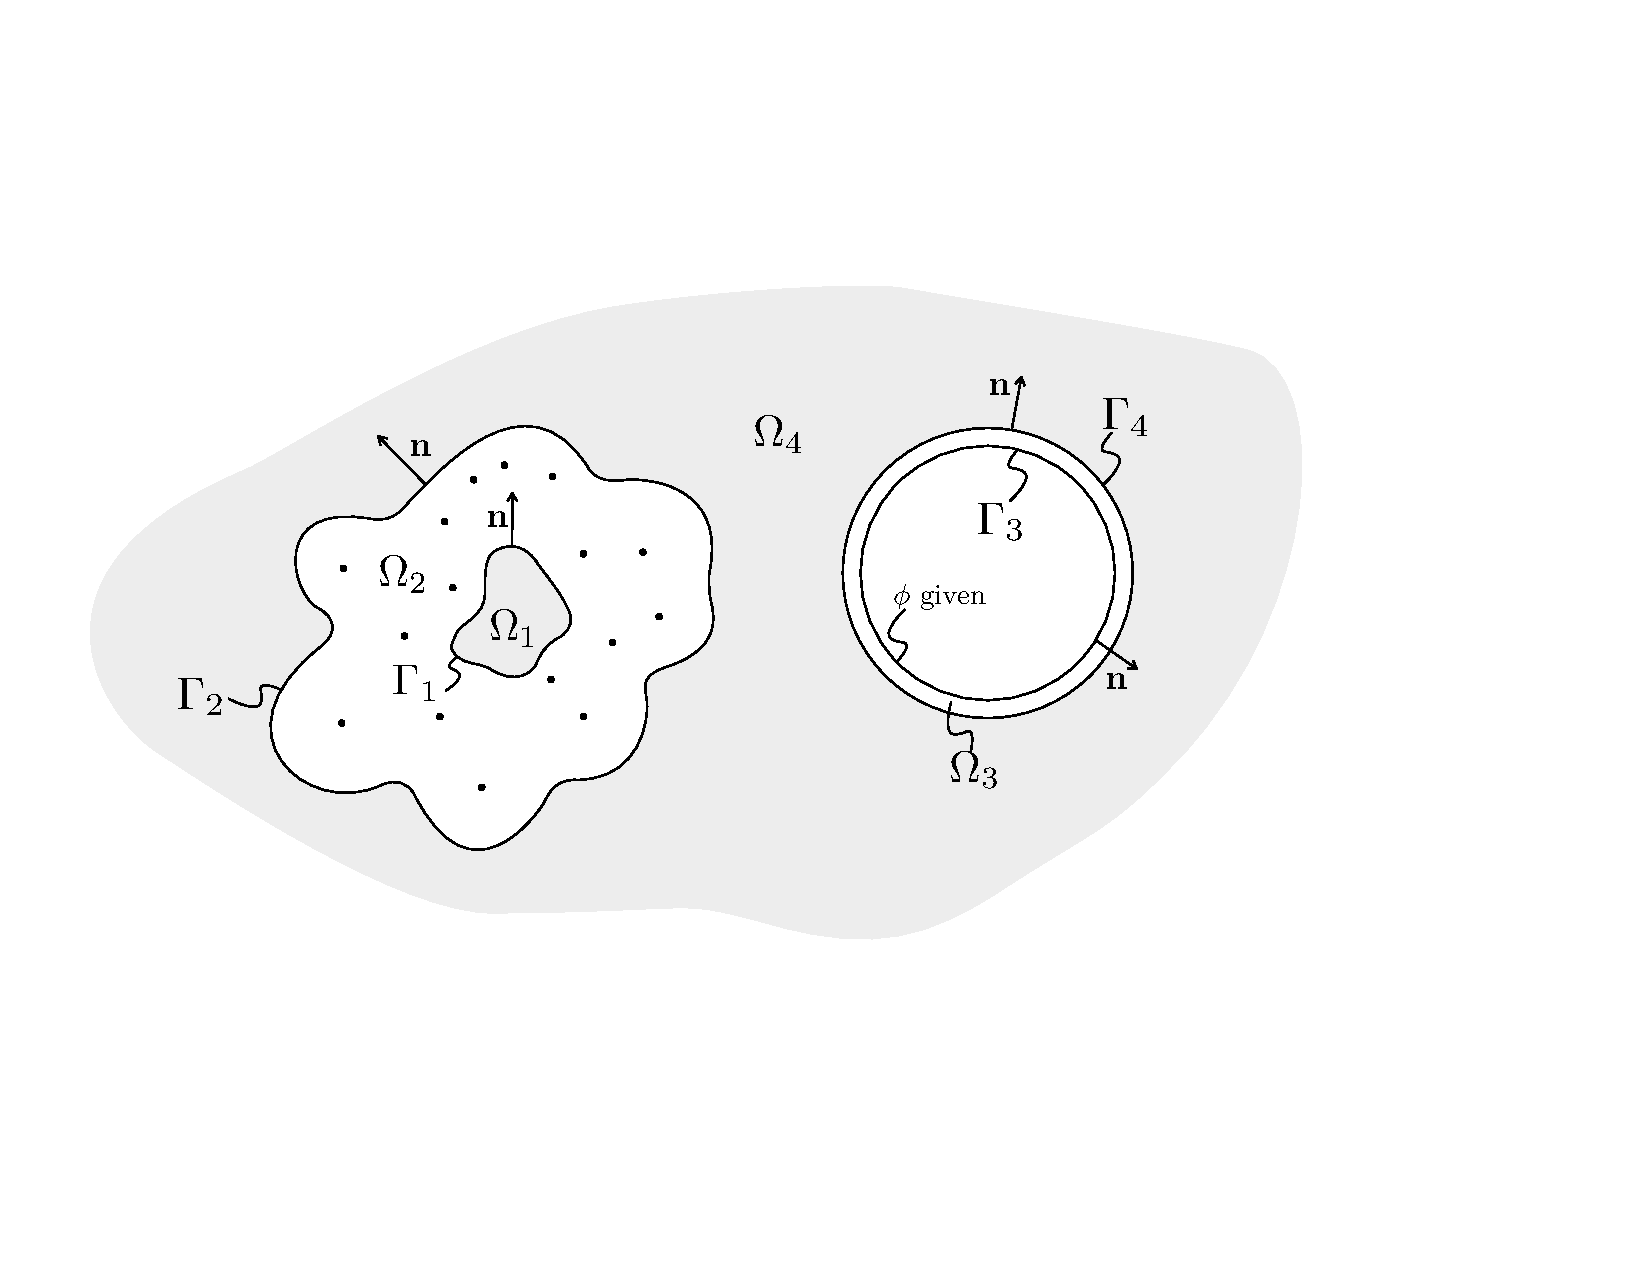
\includegraphics[width=0.5\textwidth]{molecule_surface_stern.pdf} 
   \caption{Molecule with solvent-filled cavity interacting with a surface of set potential considering a Stern layer. Gray areas are modeled by the linearized Poisson-Boltzmann equation, and white regions by the Poisson equation.}
   \label{fig:molecule_surface_stern}
\end{figure}

Even though the system in Figure \ref{fig:molecule_surface_stern} does not have many components, the matrix in Equation \eqref{eq:matrix_stern} gets considerably more complicated compared to Equation \eqref{eq:matrix_phi}. In this work, we deal with multiple surfaces following the guidelines from the work by Altman, Bardhan, White and Tidor.\cite{AltmanBardhanWhiteTidor09}

\end{comment}
%%%%===================================
